% --------------------------------------------------------------------------- %
% Poster for the ECCS 2011 Conference about Elementary Dynamic Networks.      %
% --------------------------------------------------------------------------- %
% Created with Brian Amberg's LaTeX Poster Template. Please refer for the     %
% attached README.md file for the details how to compile with `pdflatex`.     %
% --------------------------------------------------------------------------- %
% $LastChangedDate:: 2011-09-11 10:57:12 +0200 (V, 11 szept. 2011)          $ %
% $LastChangedRevision:: 128                                                $ %
% $LastChangedBy:: rlegendi                                                 $ %
% $Id:: poster.tex 128 2011-09-11 08:57:12Z rlegendi                        $ %
% --------------------------------------------------------------------------- %
\documentclass[a0paper,portrait]{baposter}

\usepackage{relsize}		% For \smaller
\usepackage{url}			% For \url
\usepackage{epstopdf}	% Included EPS files automatically converted to PDF to include with pdflatex
\usepackage{float}

%%% Global Settings %%%%%%%%%%%%%%%%%%%%%%%%%%%%%%%%%%%%%%%%%%%%%%%%%%%%%%%%%%%

\graphicspath{{pix/}}	% Root directory of the pictures 
\tracingstats=2			% Enabled LaTeX logging with conditionals

%%% Color Definitions %%%%%%%%%%%%%%%%%%%%%%%%%%%%%%%%%%%%%%%%%%%%%%%%%%%%%%%%%

\definecolor{bordercol}{RGB}{40,40,40}
\definecolor{headercol1}{RGB}{186,215,230}
\definecolor{headercol2}{RGB}{80,80,80}
\definecolor{headerfontcol}{RGB}{0,0,0}
\definecolor{boxcolor}{RGB}{186,215,230}

%%%%%%%%%%%%%%%%%%%%%%%%%%%%%%%%%%%%%%%%%%%%%%%%%%%%%%%%%%%%%%%%%%%%%%%%%%%%%%%%
%%% Utility functions %%%%%%%%%%%%%%%%%%%%%%%%%%%%%%%%%%%%%%%%%%%%%%%%%%%%%%%%%%

%%% Save space in lists. Use this after the opening of the list %%%%%%%%%%%%%%%%
\newcommand{\compresslist}{
	\setlength{\itemsep}{1pt}
	\setlength{\parskip}{0pt}
	\setlength{\parsep}{0pt}
}

%%%%%%%%%%%%%%%%%%%%%%%%%%%%%%%%%%%%%%%%%%%%%%%%%%%%%%%%%%%%%%%%%%%%%%%%%%%%%%%
%%% Document Start %%%%%%%%%%%%%%%%%%%%%%%%%%%%%%%%%%%%%%%%%%%%%%%%%%%%%%%%%%%%
%%%%%%%%%%%%%%%%%%%%%%%%%%%%%%%%%%%%%%%%%%%%%%%%%%%%%%%%%%%%%%%%%%%%%%%%%%%%%%%

\begin{document}
\typeout{Poster rendering started}

%%% Setting Background Image %%%%%%%%%%%%%%%%%%%%%%%%%%%%%%%%%%%%%%%%%%%%%%%%%%
\background{
	\begin{tikzpicture}[remember picture,overlay]%
	\draw (current page.north west)+(-2em,2em) node[anchor=north west]
	{
\includegraphics[height=1.1\textheight]{background}};
	\end{tikzpicture}
}

%%% General Poster Settings %%%%%%%%%%%%%%%%%%%%%%%%%%%%%%%%%%%%%%%%%%%%%%%%%%%
%%%%%% Eye Catcher, Title, Authors and University Images %%%%%%%%%%%%%%%%%%%%%%
\begin{poster}{
	grid=false,
	% Option is left on true though the eyecatcher is not used. The reason is
	% that we have a bit nicer looking title and author formatting in the headercol
	% this way
	%eyecatcher=false, 
	borderColor=bordercol,
	headerColorOne=headercol1,
	headerColorTwo=headercol2,
	headerFontColor=headerfontcol,
	% Only simple background color used, no shading, so boxColorTwo isn't necessary
	boxColorOne=boxcolor,
	headershape=roundedright,
	headerfont=\Large\sf\bf,
	textborder=rectangle,
	background=user,
	headerborder=open,
  boxshade=plain
}
%%% Eye Cacther %%%%%%%%%%%%%%%%%%%%%%%%%%%%%%%%%%%%%%%%%%%%%%%%%%%%%%%%%%%%%%%
{
	Eye Catcher, empty if option eyecatcher=false - unused
}
%%% Title %%%%%%%%%%%%%%%%%%%%%%%%%%%%%%%%%%%%%%%%%%%%%%%%%%%%%%%%%%%%%%%%%%%%%
{\sf\bf
	Spatial Frequency Modulated Imaging (SPIFI)
}
%%% Authors %%%%%%%%%%%%%%%%%%%%%%%%%%%%%%%%%%%%%%%%%%%%%%%%%%%%%%%%%%%%%%%%%%%
{
	\vspace{1em} Brennan W. Fieck
}
%%% Logo %%%%%%%%%%%%%%%%%%%%%%%%%%%%%%%%%%%%%%%%%%%%%%%%%%%%%%%%%%%%%%%%%%%%%%
{
% The logos are compressed a bit into a simple box to make them smaller on the result
% (Wasn't able to find any bigger of them.)
\setlength\fboxsep{0pt}
\setlength\fboxrule{0.5pt}
	\fbox{
		\begin{minipage}{10em}
			
\includegraphics[width=10em]{pix/Piercing Gaze Logo.png}
		\end{minipage}
	}
}

\headerbox{Abstract}{name=problem,column=0,row=0}{
This team's project was primarily to provide simulation software to compare the output predicted by an ideal system to actual data collected from these systems once they have been constructed, and to produce software to implement photon counting on the output of SPIFI systems. The advantage of 2D SPIFI is to enable the system to scan the object much faster by eliminating the current need to scan over the object by expanding the spatial frequency modulation. The advantage of photon-counting is that one can immediately resolve which part of an object a particular photon scanned, eliminating the need to do some signal processing on SPIFI signals.
}

\headerbox{Background}{name=definitions,column=0,below=problem}{
SPIFI is a revolutionary imaging technique that allows a line to be scanned
across an object by a single laser at one time, without using a raster pattern
along the line. In particular, it is impressive because a full,
two-dimensional image can be extracted from light collected at a single
point. Traditionally, scanning more than a single point at a time
would require multiple collectors to be able to
resolve which photons were used to scan what part of the object (e.g.
using a camera). SPIFI enables scientists to scan objects with one
collector by encoding this information in a
frequency change that maps directly to a line on the object.
The focus of this project is to expand the capabilities of SPIFI by adding another
dimension to this encoding.
\begin{centering}
	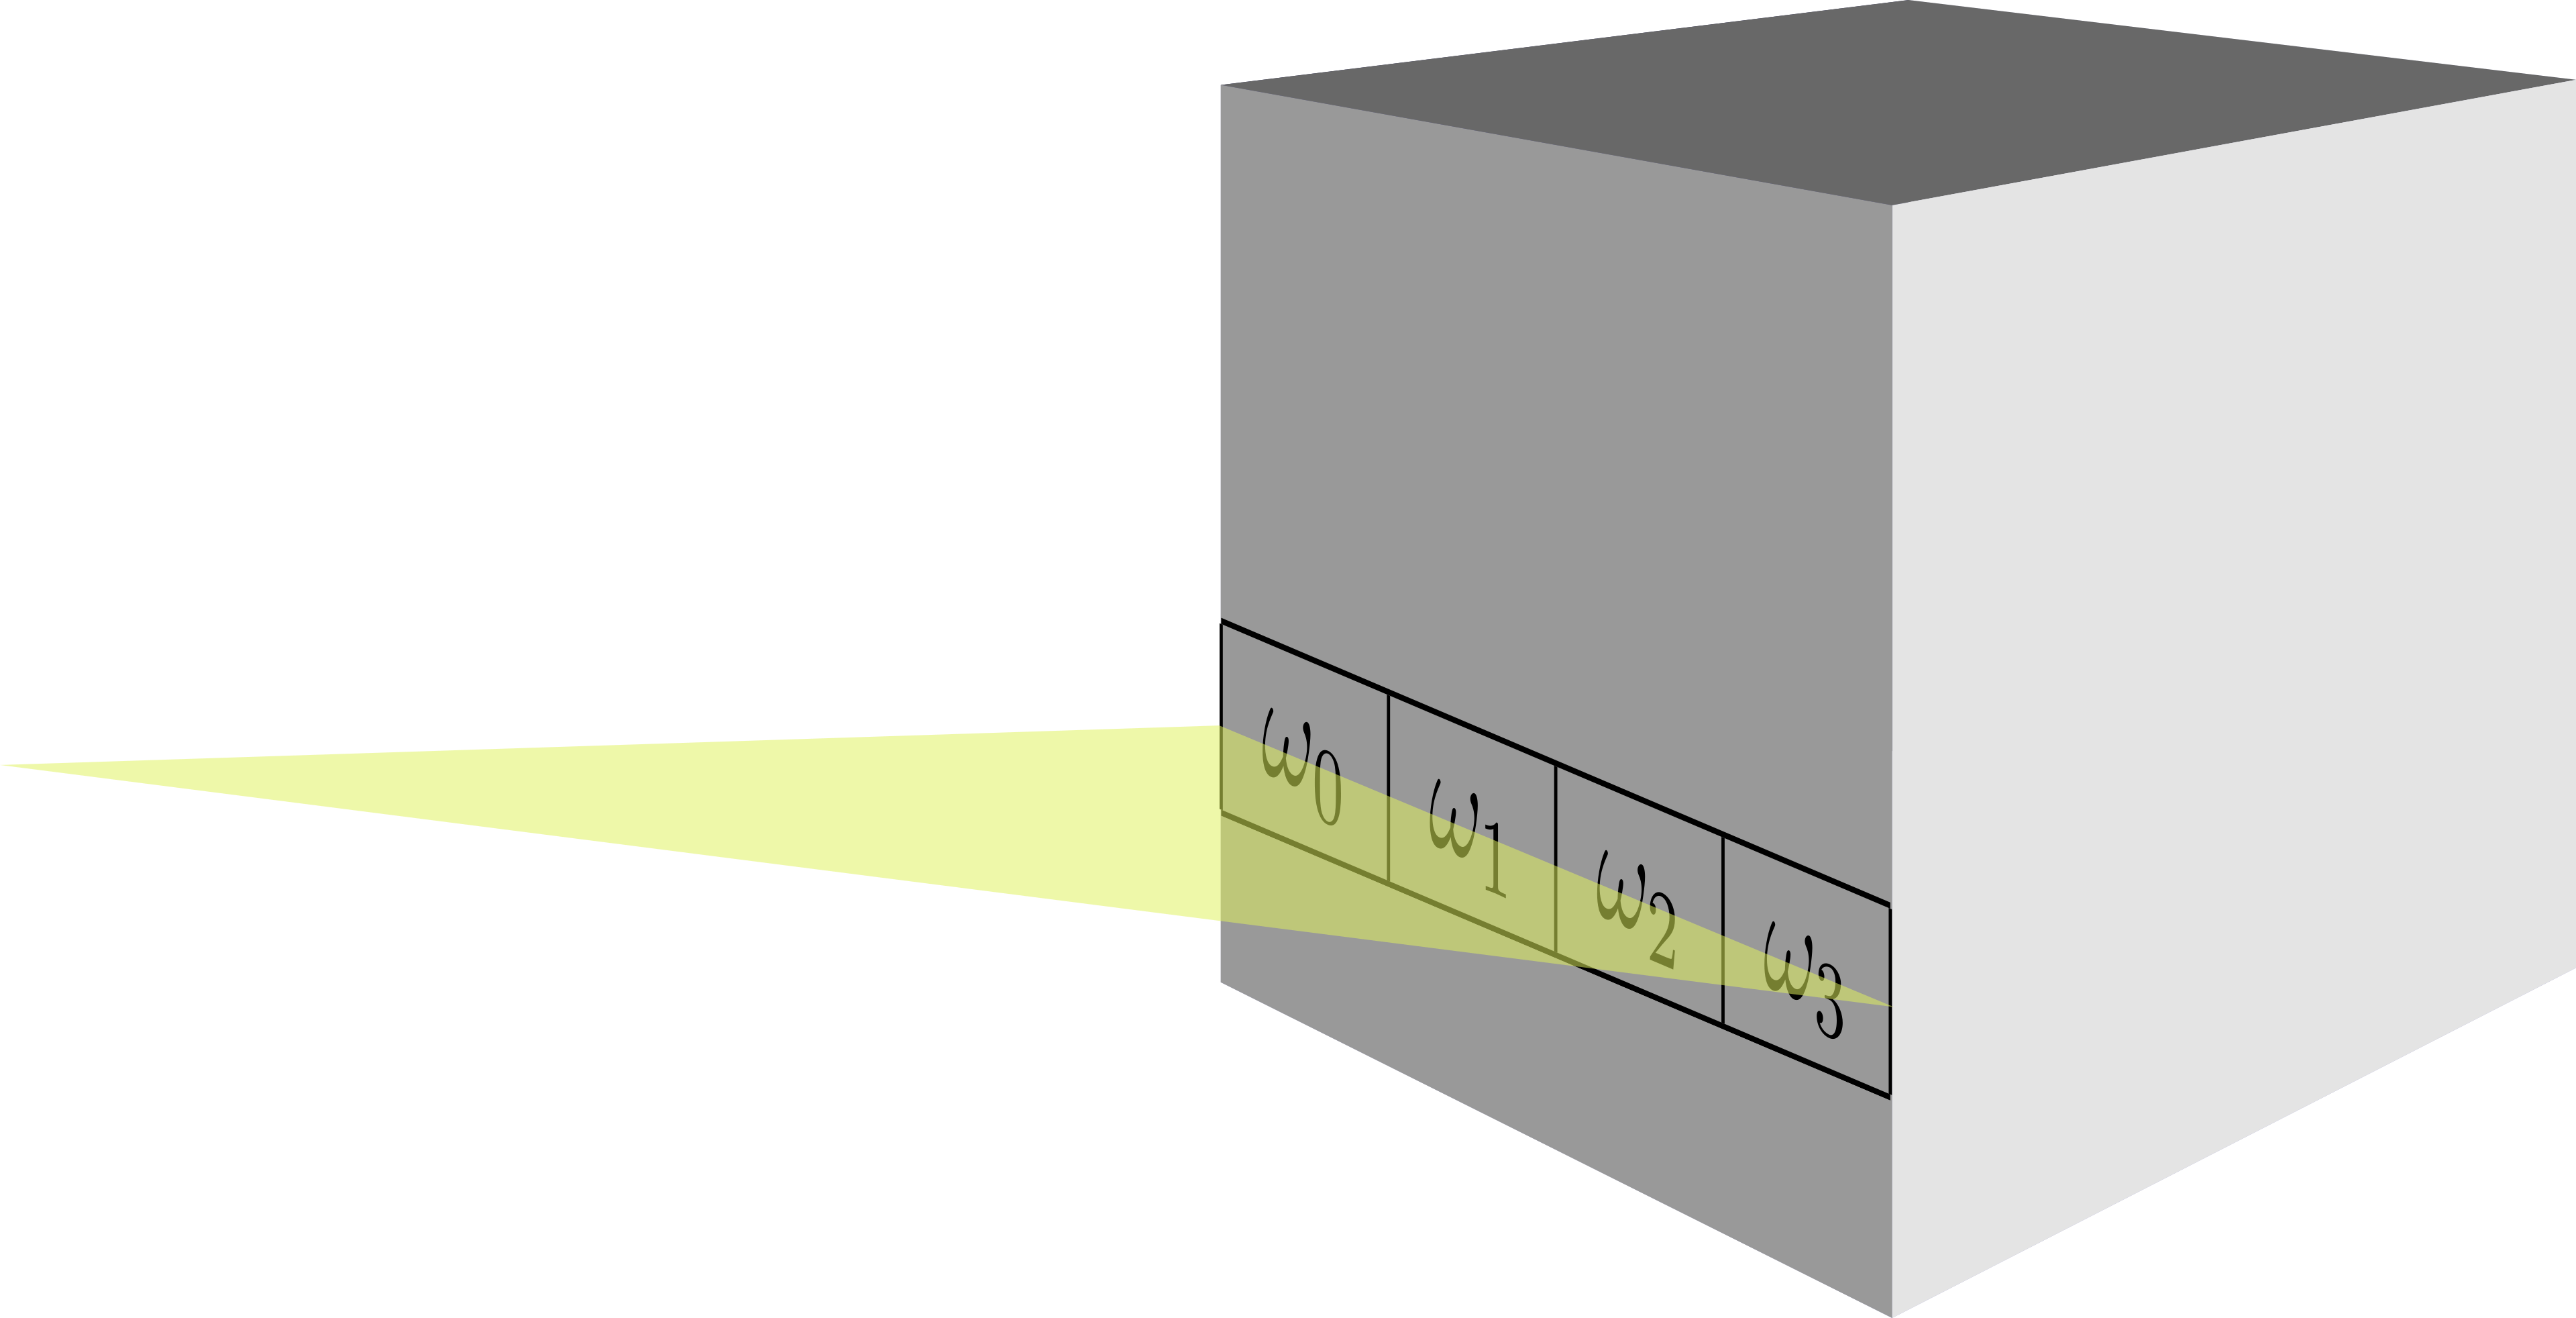
\includegraphics[width=\textwidth]{pix/spifi-system}
\end{centering}

}

\headerbox{References}{name=references,column=0,below=definitions,above=bottom}{
\smaller													% Make the whole text smaller
\vspace{-0.4em} 										% Save some space at the beginning
\bibliographystyle{plain}							% Use plain style
\renewcommand{\section}[2]{\vskip 0.05em}		% Omit "References" title
\begin{thebibliography}{9}

\bibitem{lamport94}
  Dr Jeff Squier. Dr Keith Deluca. et. al.
  \emph{Super-Resolved Multimodal Multiphoton Microscopy with Spatial Frequency-Modulated
Imaging},
  Proceedings of the National Academy of Sciences,
  2015.

\bibitem{boreman}
	Glenn D. Boreman et. al.
	\emph{Use of spatial light modulators in frequency modulation reticle trackers},
	Optical Engineering, November 1990

\bibitem{nih}
	Jeff A. Squier. Michael D. Young. et. al.
	\emph{Eliminating the scattering ambiguity in multifocal, multimodal multiphoton imaging systems},
	J Biophotonicts. 2012 May

\bibitem{micro}
	Michael D. Young.
	"Microfluidic Projection Mask Imaging"
	Colorado School of Mines, Golden. October 20, 2016. Presentation.

\bibitem{Fourier}
	Nicholas George,
	"Fourier Optics," M.S. thesis, Hajim School of Engineering \& Applied Science, University of Rochester, Rochester, NY, 2012

  
\bibitem{talk}
  Futia, Greg. Winters, Dave. Schlup, Philip. Bartels, Dr Randy.
  "Spatial Frequency Modulated Imaging on a Single Element Detector."
  Colorado School of Mines, Golden. May 24, 2011. Presentation.
  

\end{thebibliography}
}

\headerbox{2D SPIFI}{name=density,span=2,column=1,row=0}{
Current SPIFI techniques require scanning across an object by physically "wobbling" a mirror. 2D SPIFI would not only remove this requirement, but would allow one to scan the entire object at once, providing an $O[n]$ decrease in the time necessary to scan an object.\\
\begin{centering}
	\begin{minipage}{0.48\linewidth}
		\vspace{-10em}
		This basically amounts to another rotating SPIFI mask, but rather than a linear pattern, it would encode along it entire "sub-masks" so that the laser beam could be spread out into a plane instead of just a line. Essentially this replacing temporal encoding of frequency (pictured right) used in 1D SPIFI with a spatial encoding. It's actually quite analogous to the idea of 1D SPIFI as opposed to raster scans.
	\end{minipage}
	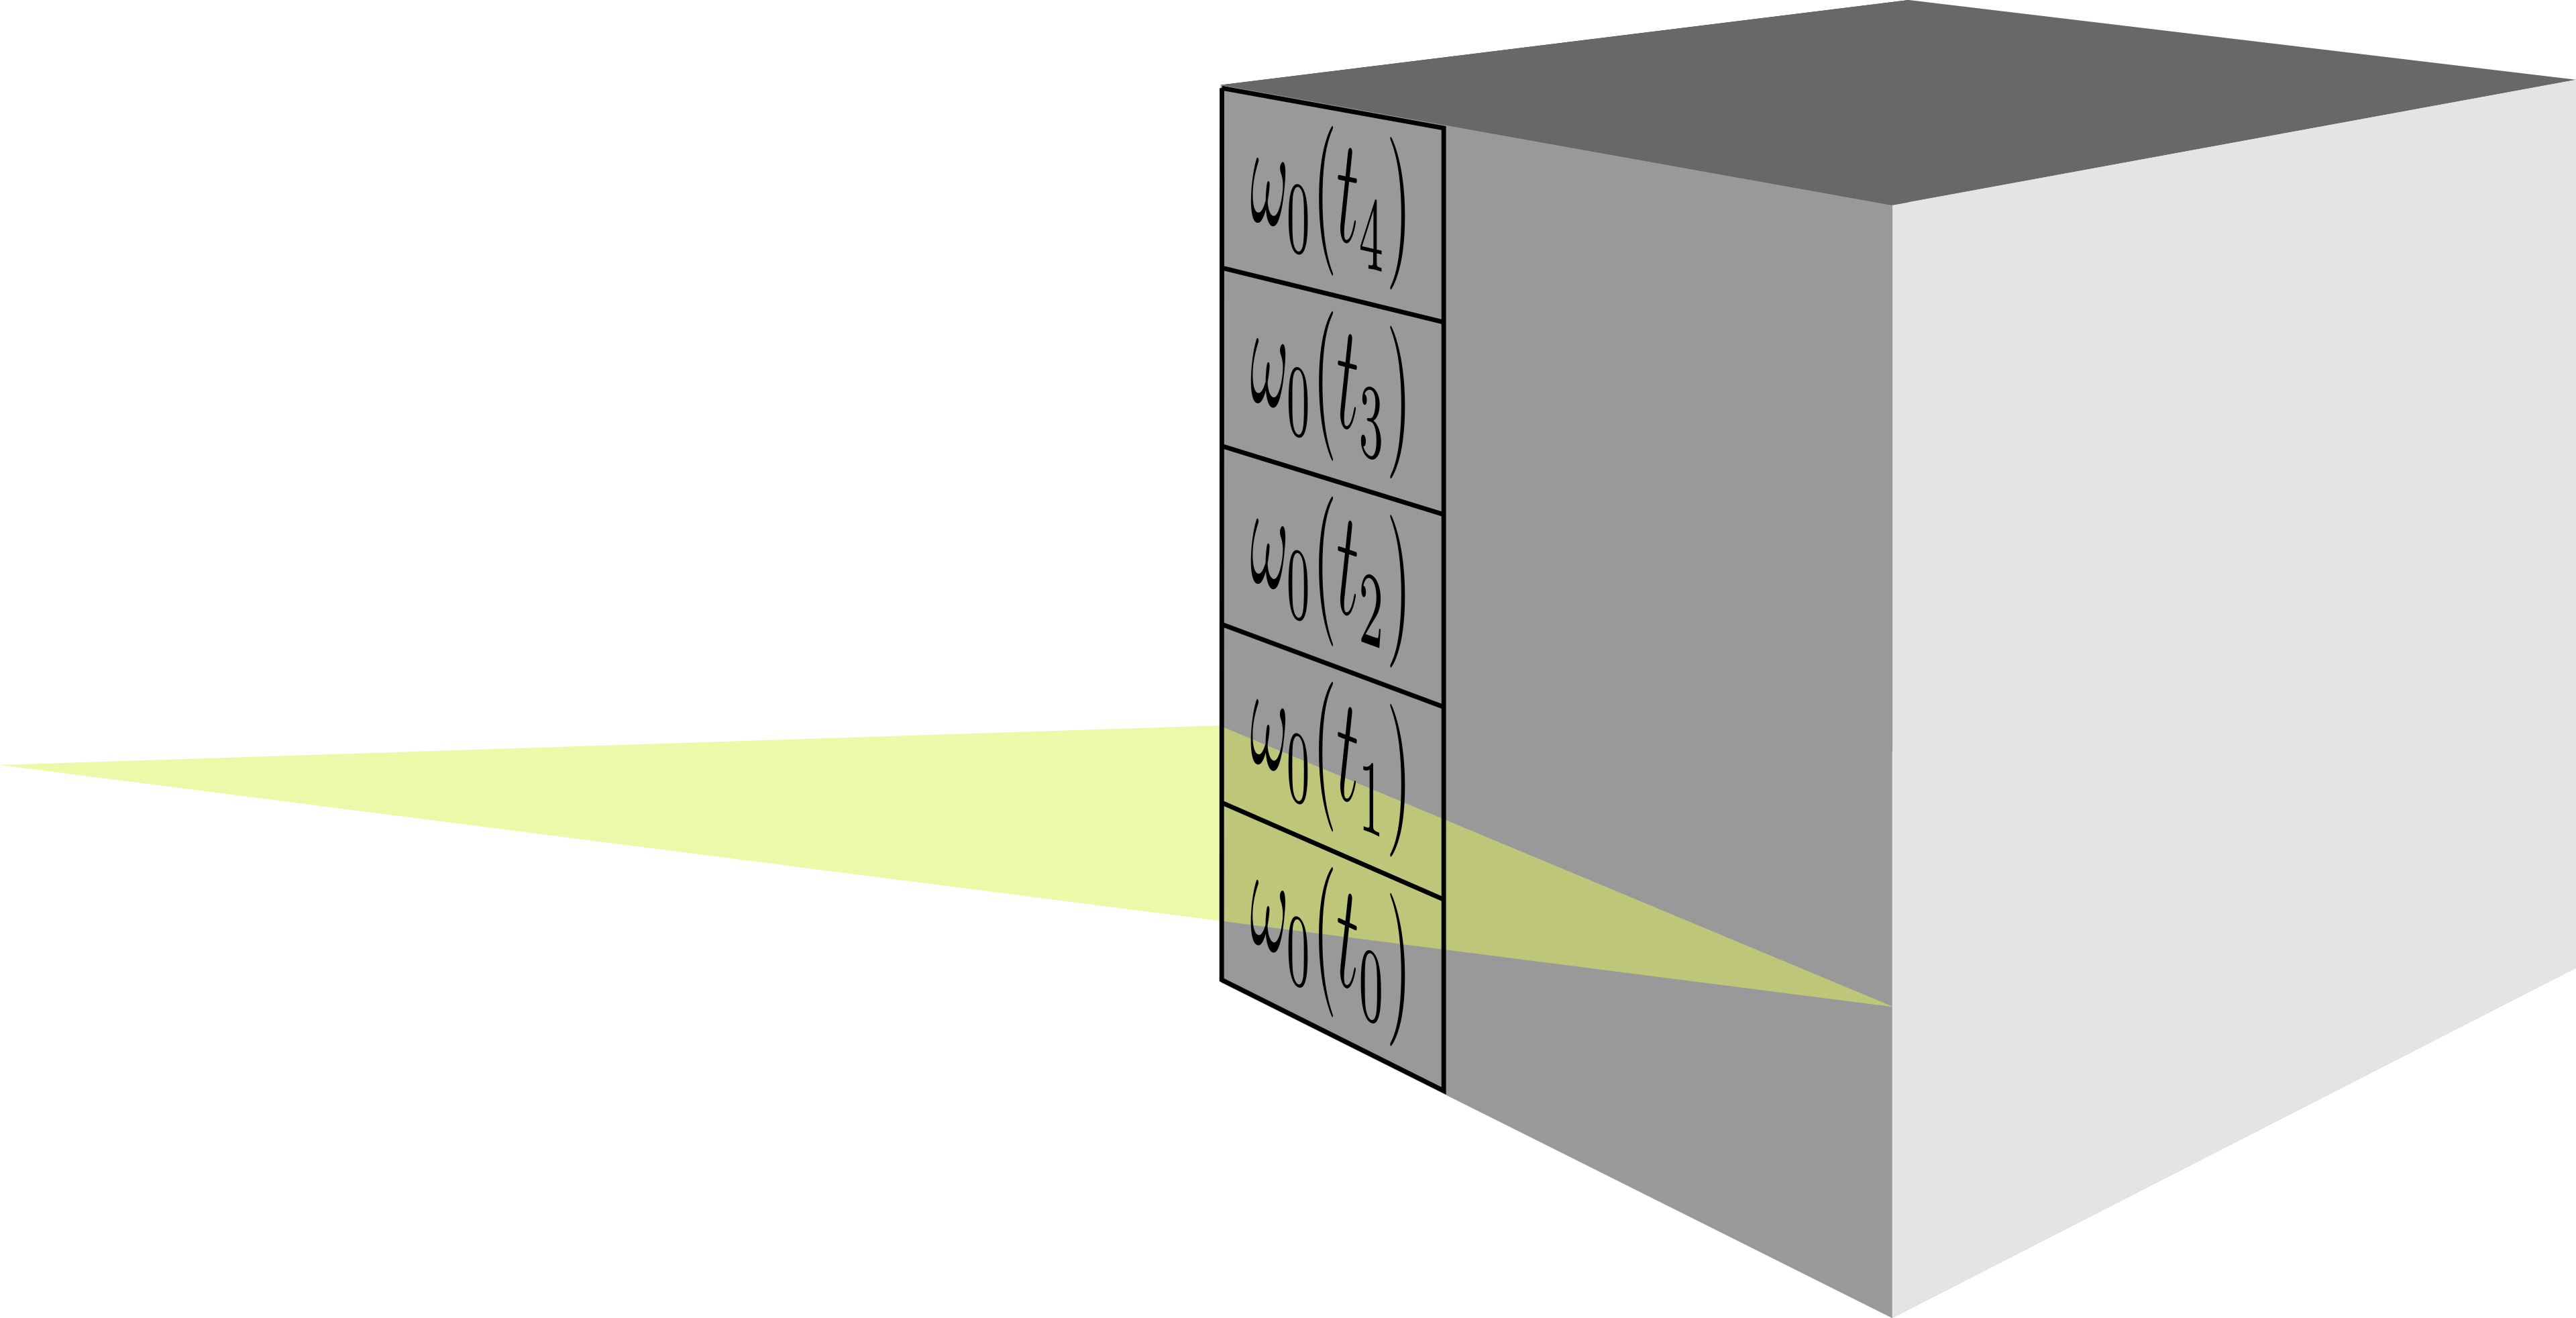
\includegraphics[width=0.48\linewidth]{pix/spifi-sheet}
\end{centering}\\
This team wrote software which simulated this 2-dimensional SPIFI technique as a proof-of-concept, as well as an aid to test designs for 2D SPIFI masks. Shown below is the effective spatial frequency mapping used by 2D SPIFI, alongside an input and corresponding output of the simulator (using image files as objects).\\
\begin{figure}[H]
	\centering
	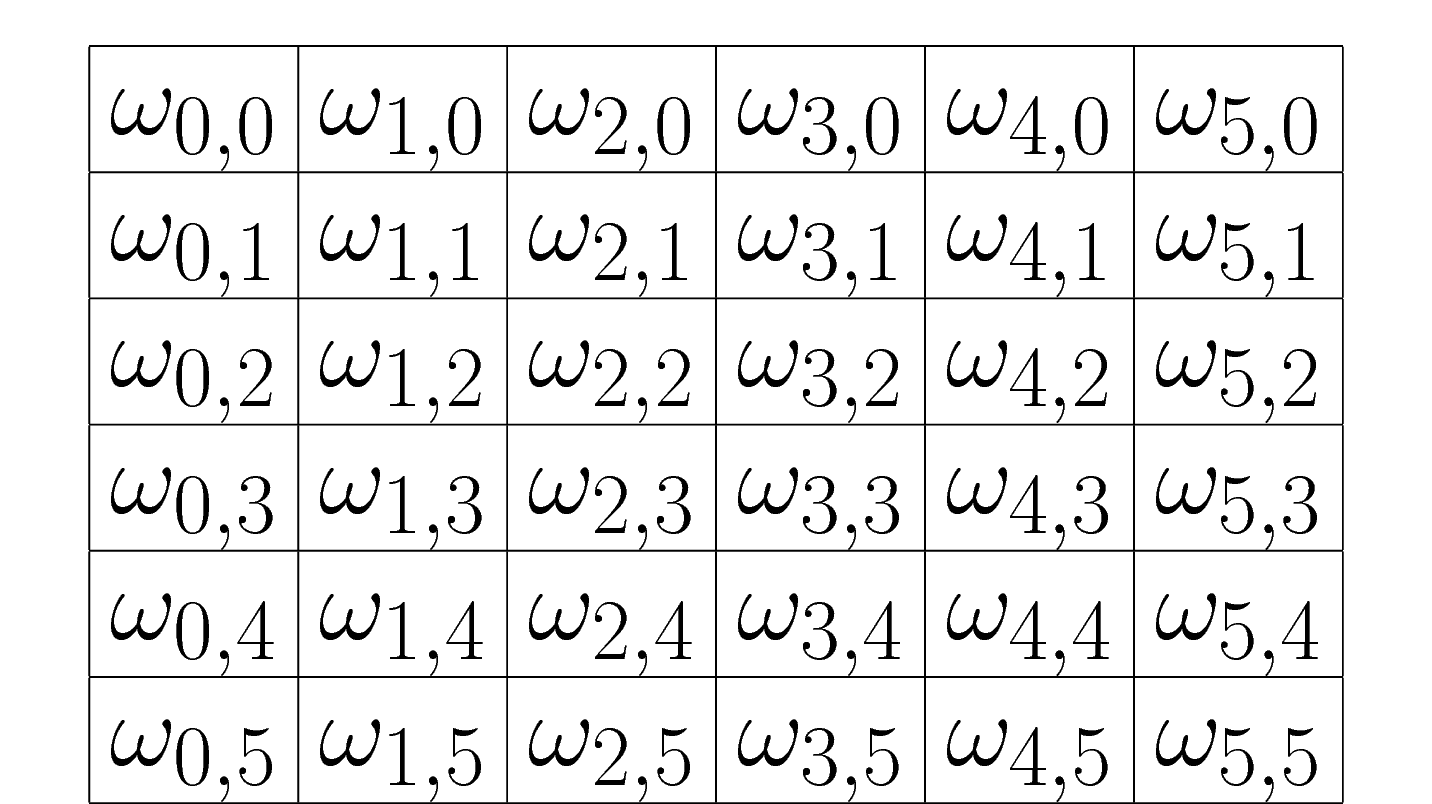
\includegraphics[width=0.32\textwidth,height=12em]{pix/spifi-grid}
	
\includegraphics[width=0.32\textwidth,height=12em]{pix/testimg}
	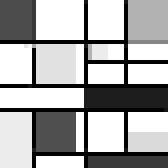
\includegraphics[width=0.32\textwidth,height=12em]{pix/testoutput}
	\caption{Left: Effective Spatial Frequency of 2D SPIFI - Center: Sample Simulation Input - Right: Sample Simulation Output}
\end{figure}
}

\headerbox{Photon Counting}
{name=degreeDistribution,span=2,column=1,below=density}{
Photon counting refers to analyzing the collected output of a SPIFI system (1D or 2D; both can utilize photon counting) to resolve the detection of individual photons. Photon counting improves the sensitivity of our detection as a function of time. The signal must still be transformed to extract the final image. The detection is a simple enough process that it can be performed on a micro-controller or field-programmable gate array (FPGA). The actual hardware chosen was an Altera$^\textnormal{TM}$ DE0-Nano FPGA. Shown below is a sample timing diagram showing how individual photons can be related to bursts of the laser.\\
\begin{figure}[H]
	\centering
	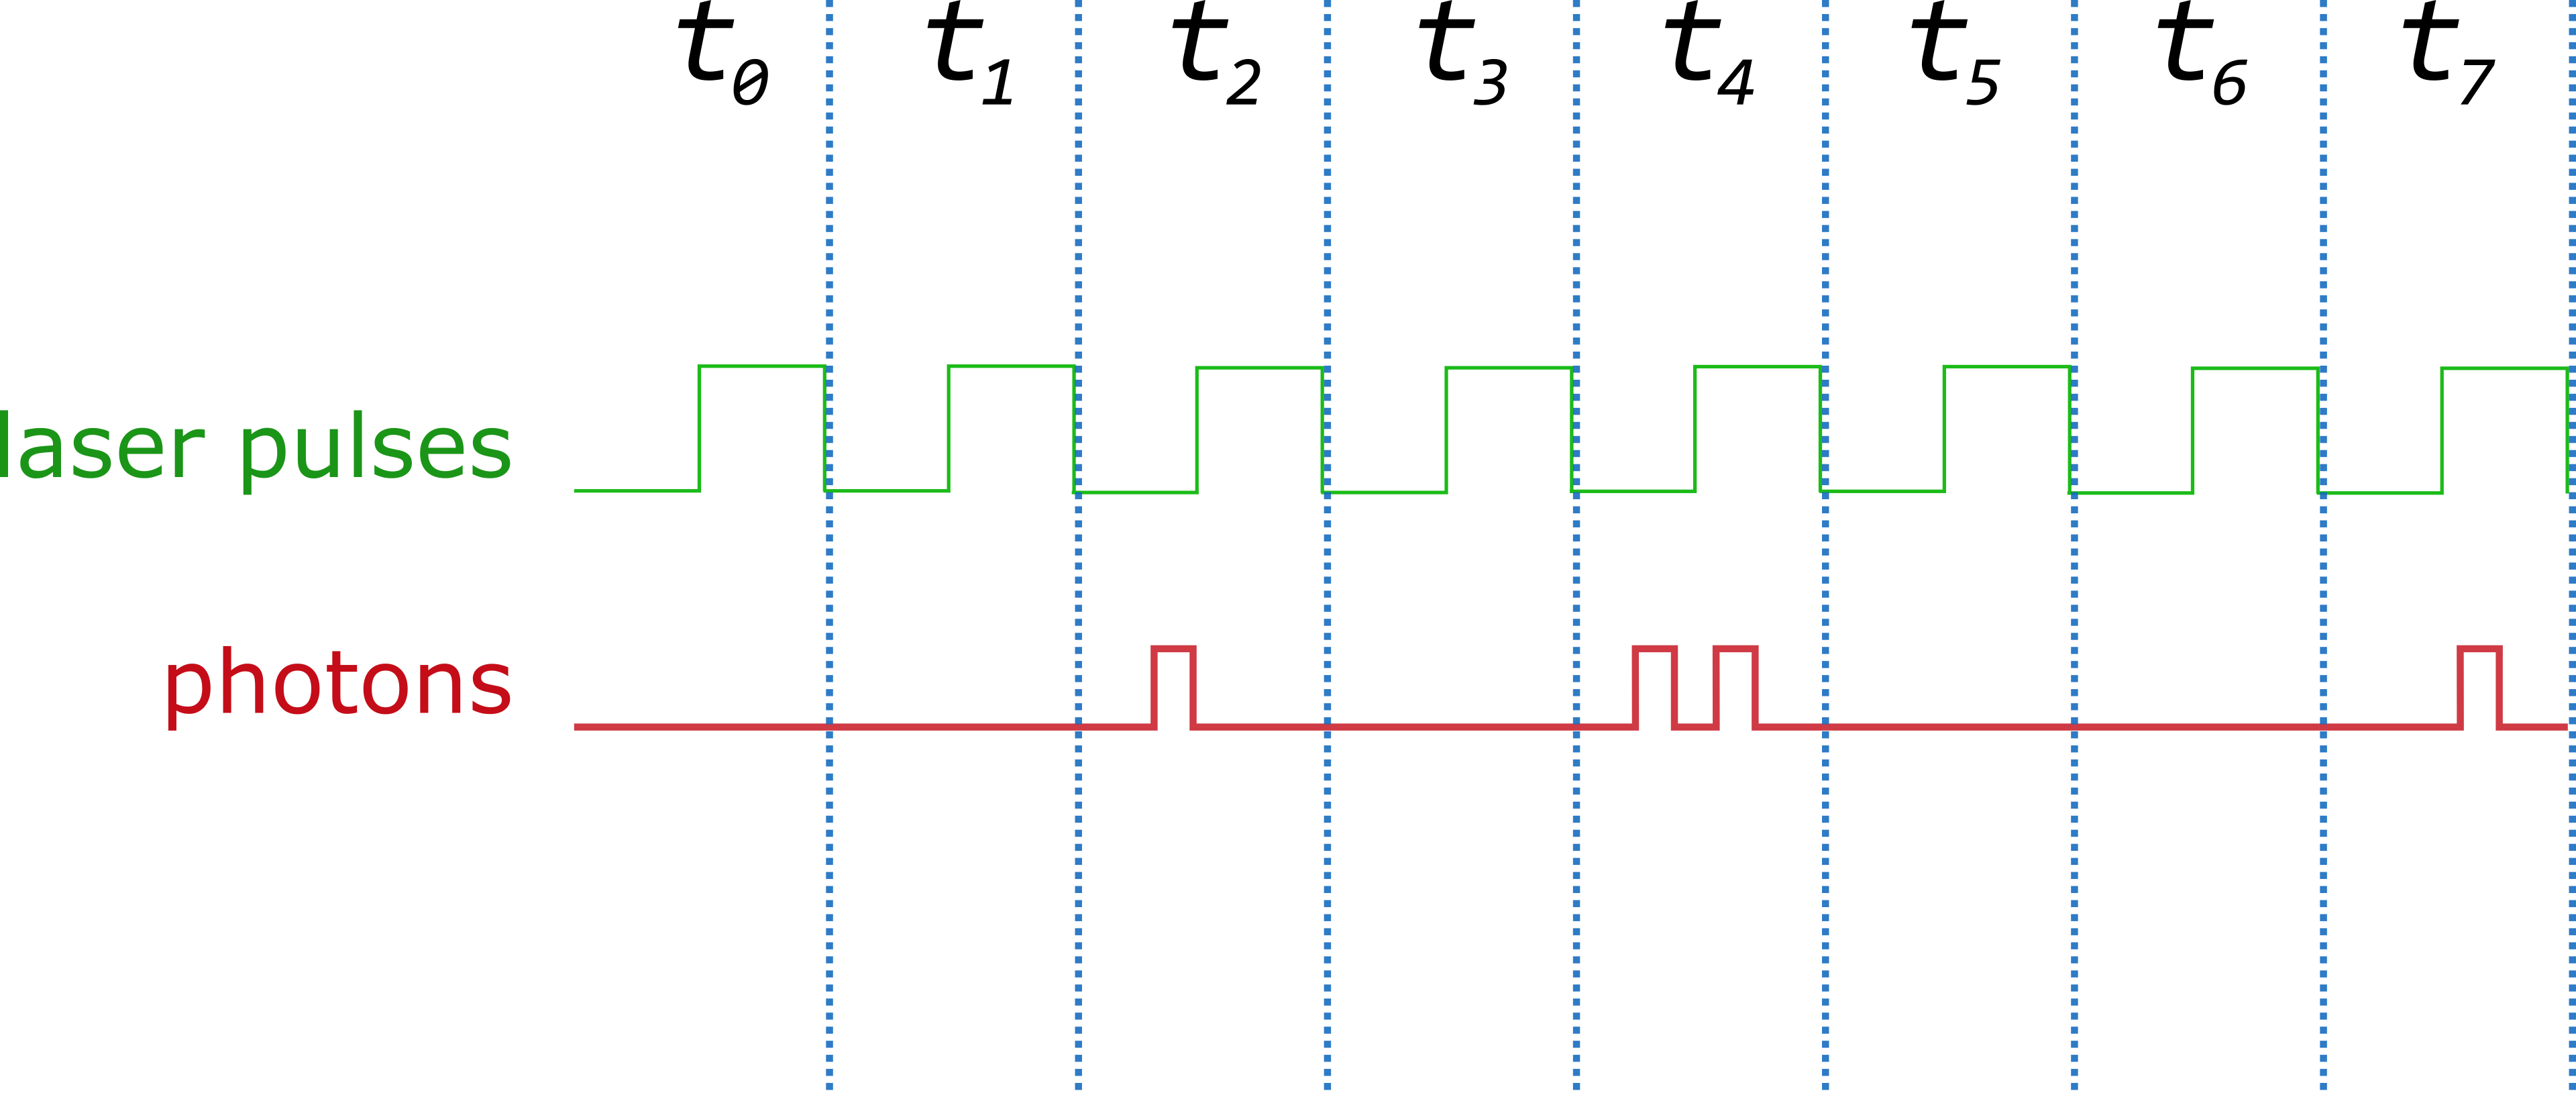
\includegraphics[width=0.7\textwidth]{pix/sample-timing-diagram}
\end{figure}
}

\headerbox{Software Notes}
{name=notes,span=2,column=1,below=degreeDistribution,above=bottom}{
	Unfortunately, the research is still pending publication. At the time of publication, the source will be made available to the community along with its respective documentation.
Once released, the software is provided under the GNU Public License version 3. The simulation is written in the open Python 3.5.2 standard, with a list of free and open source dependencies that will be made available at the same time as the simulation itself. The FPGA code was written using the Quartus software which is the property of Altera$^\textnormal{\small TM}$, along with various pieces of supporting software each of which is subject to its own license.
}

\end{poster}
\end{document}
